\chapter{IPSec: IP Security}
IPSec è un altro protocollo di sicurezza che non lavora più sul garantire una sessione sicura, ma si impegna per proteggere \textbf{tutto} il pacchetto IP. Spesso il protocollo viene associato alle VPN, in quanto ne permette la costruzione. Ne vedremo poi una parentesi.
\section{Protocol Structure}
Il protocollo IPSec è detto anche \textbf{Network Layer Security} ed è un protocollo di \textbf{livello di rete} (livello 3) nell'architettura TCP/IP, che permette di \textbf{proteggere} sia l'\textbf{header} che il \textbf{payload} dei pacchetti IP. La protezione è quindi direttamente sull'\textbf{host} e basta sugli \textbf{indirizzi IP}.\\
Può essere implementato nei seguenti modi:
\begin{theorem}[IPSec implementation]
\noindent\begin{itemize}
    \item \textbf{Native IP Code:}  viene incluso all'interno del protocollo IP. Tipico delle soluzioni UNIX.
    \item \textbf{BITS (Bump in The Stack):} viene implementato come \textbf{protocollo intermedio} tra il livello di rete (protocollo IP) ed il livello di collegamente, agendo come driver intermedio.
    \item \textbf{BITW (Bump in The Wire):} viene implementato all'interno della \textbf{NIC} (Network Interface Card) del sistema dell'host, ovvero all'interno dell'\textbf{hardware}.
\end{itemize}
\end{theorem}
\begin{remark}
IPSec \textbf{coopera} e \textbf{coesiste} con il protocollo IP, per cui nella \textbf{comunicazione} tra due hosts vengono utilizzati sia \textbf{pacchetti IP protetti} da \textbf{IPsec} che \textbf{pacchetti IP non protetti}. E' inoltre \textbf{trasparente al livello applicativo} e non può proteggere direttamente le applicazioni.
\end{remark}
\begin{figure}[h]
    \centering
    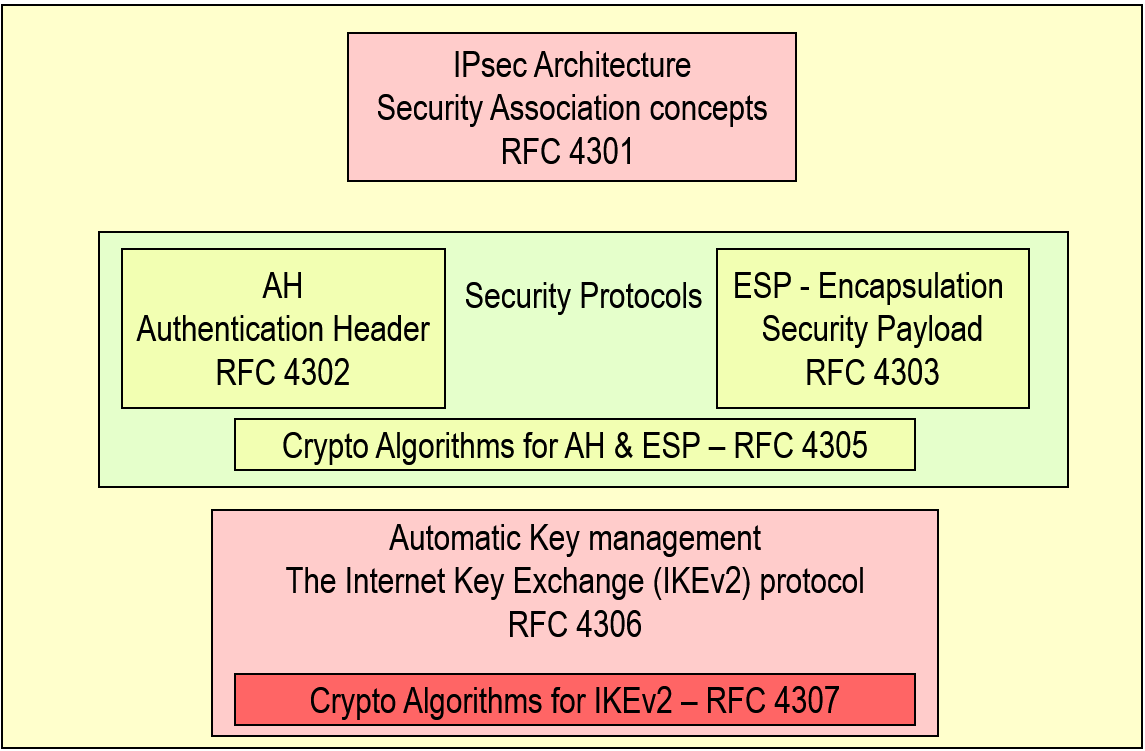
\includegraphics[width=0.7\textwidth]{image/ipsec.png}
    \caption{IPSec Architecture}
    \label{fig:ipsecarc}
\end{figure}
\pagebreak
\begin{definition}[IPSec Architecture]\label{def:ipsecarc}
Nel protocollo IPSec distinguiamo le seguenti componenti: (\cref{fig:ipsecarc})
\begin{itemize}
    \item \textbf{Security Association:} identifica una connessione da un host mittente ad un host destinario. Definisce perciò l'architettura della comunicazione tra hosts.
    \item \textbf{Security Protocols:} protocolli per il trasferimento dei dati che garantiscono specifiche proprietà di sicurezza.
    \item \textbf{Key Management:} protocolli per l’instaurazione della connessione tra due hosts.
\end{itemize}
\end{definition}
\subsection{Security Association}
\textbf{Una Security Association (SA)} rappresenta una \textbf{connessione unidirezionale sicura} tra un \textbf{IP mittente} ed un \textbf{IP destinatario}, ovvero \textbf{definisce} i \textbf{confini} \textbf{entro i quali} i \textbf{pacchetti IP} vengono \textbf{protetti tramite criptazione e autenticazione}. Tali confini possono essere:
\begin{itemize}
    \item Host to Host.
    \item Host to Intermediete Router (security Gateway).
    \item Security Gateway to Security Gateway.
\end{itemize}
\begin{note}
Nella SA non c'è trasmissione dati, ma soltanto una serie di azioni per inizializzare parametri di sicurezza.
\end{note}
\begin{proposition}[SA Setup]\label{prop:sasetup}
Le SA forniscono dei meccanismi di configurazione di due tipi:
\begin{itemize}
    \item \textbf{Manualmente:} tutti i parametri della SA sono configurati in maniera manuale. Ne deriva che tale metodo è adatto solamente per VPN di piccole dimensioni.
    \item \textbf{Automaticamente:} vengono gestite tramite il protocollo IKEv2. In particolare, è possibile generare nuove SA su richiesta e gestire i parametri di sicurezza per sessioni.
\end{itemize}
\end{proposition}
Per poter gestire le SA e il traffico di dati, ogni entità mantiene:

\begin{definition}[Un Security Association Database (SAD)]\label{def:sad}
Il \textbf{SAD mantiene} le \textbf{informazioni} delle \textbf{SA attive} sia per il traffico entrante che uscente dall’entità. Per ogni SA \textbf{vengono memorizzati} i seguenti parametri:
\begin{itemize}
    \item \textbf{Security Parameters Index (SPI):} (32 bits) \textbf{identifica} univocamente la SA.
    \item \textbf{Lifetime:} tempo di vita della SA:
    \item \textbf{Indirizzo di Origine:} indirizzo \textbf{IP} del \textbf{mittente}
    \item \textbf{Indirizzo di Destinazione:} indirizzo \textbf{IP} del \textbf{destinatario}.
    \item \textbf{Security Protocol:} protocollo di sicurezza IPsec utilizzato per la SA.
    \item \textbf{Sequence Number Counter:} numero di sequenze per i pacchetti IPsec inviati sulla SA.
    \item \textbf{Anti-Replay Window:} definisce la finestra di pacchetti per la quale vengono contrastati replay attacks.
    \item \textbf{Algoritmi:} algoritmi utilizzati dalla SA per la criptazione ed il controllo di integrità.
    \item \textbf{Chiavi:} chiavi simmetriche utilizzate dalla SA per la criptazione ed il controllo di integrità.
\end{itemize}
\end{definition}

\begin{definition}[Un Security Policy Database (SPD)]\label{def:spd}
L'\textbf{SPD} \textbf{mantiene un insieme di Security Policy (SP)} per determinare le modalità con le quali un pacchetto che transita attraverso l’entità deve essere processato. In particolare, l’insieme di regole espresse all’interno del SPD permette di determinare se un pacchetto debba essere:
\begin{itemize}
    \item \textbf{Ignorato:} il pacchetto IP/IPsec in transito \textbf{non} deve essere \textbf{elaborato} dal \textbf{protocollo IPsec}.
    \item \textbf{Protetto:} il pacchetto IP/IPsec \textbf{deve} essere \textbf{elaborato} dal \textbf{protocollo IPsec.}
    \item \textbf{Scartato:} il pacchetto IP/IPsec \textbf{deve} essere \textbf{scartato/bloccato} dall’entità.
\end{itemize}
Per i Pacchetti \textbf{protetti da IPsec}, il SPD definisce le modalità di elaborazione in funzione delle caratteristiche del pacchetto (header IP e relazioni con il traffico di rete). Alcune di queste modalità sono:
\begin{itemize}
    \item Quale \textbf{protocollo di sicurezza IPsec} deve essere utilizzato e con quale \textbf{modalità}.
    \item La \textbf{granularità} con la quale devono essere gestiti i pacchetti.
    \begin{itemize}
        \item Un \textbf{singolo Tunnel} condiviso per \textbf{tutte le connessioni}.
        \item Un \textbf{tunnel} \textbf{per ogni} diferente connessione TCP.
    \end{itemize}
\end{itemize}
\end{definition}
\subsection{Security Protocol}
IPsec prevede due differenti protocolli di sicurezza:
\begin{definition}[Authentication Header]\label{def:ah}
Sia su payload che header dei pacchetti IP viene fatto controllo di integrità inserendo un tag tra IP header e payload. \\
Viene fornita \textbf{protezione} contro \textbf{replay attacks}
\end{definition}
\begin{definition}[Encapsulated Security Payload]
Viene fornita autenticazione e confidenzialità con AEAD del \textbf{solo payload} del pacchetto IP, che viene rinchiuso da un nuovo header (inserito tra header e payload) e da un trailer più tag di auth.\\
Viene \textbf{fornita} protezione \textbf{contro replay attacks} e \textbf{traffic flow confidentiality}.
\end{definition}
\begin{remark}
Nelle ultime RFC AH è stato declassato da \textit{"Must"} a \textit{"May"} poiché è stato visto che ESP copre la maggior parte dei requisiti necessari ai servizi di sicurezza. Raramente vengono usate anche in combinazione.
\end{remark}
IPsec ha la caratteristica di poter operare in due modalità differenti:
\begin{definition}[IPsec Transport]\label{def:transport}
Il pacchetto IP protetto da IPsec viene elaborato direttamente dall'host.\\
\begin{remark}
Se viene usato AH e l'ip viene cambiato il pacchetto viene scartato.
\end{remark}
\end{definition}\pagebreak
\begin{definition}[IPsec Tunnel]\label{def:tunnel}
Il pacchetto IP protetto da IPsec viene \textbf{incapsulato all'interno di un altro pacchetto IP} dopo aver aggiunto un tag che protegge tutto il pacchetto.\\
\begin{remark}
In tunneling l'IP del pacchetto che viene consegnato è quello del tunnel ed è diverso da quello realmente creato a livello di trasporto.
\end{remark}
\end{definition}
La modalità di lavoro del protocollo viene determinata in base all'esigenza dell'applicazione:
\begin{theorem}[IPsec mode selection]\label{def:ipsecmodesel}
\begin{itemize}
    \item \textbf{Transport Mode} per connessioni \textbf{host-to-host} o \textbf{host-to-gateway}. In alcuni casi anche per connessioni \textbf{gateway-to-end} o \textbf{end-to-gateway}
    \item \textbf{Tunnel Mode} per connessioni \textbf{gateway-to-gateway}.
\end{itemize}
\end{theorem}
\begin{figure}[h]
    \centering
    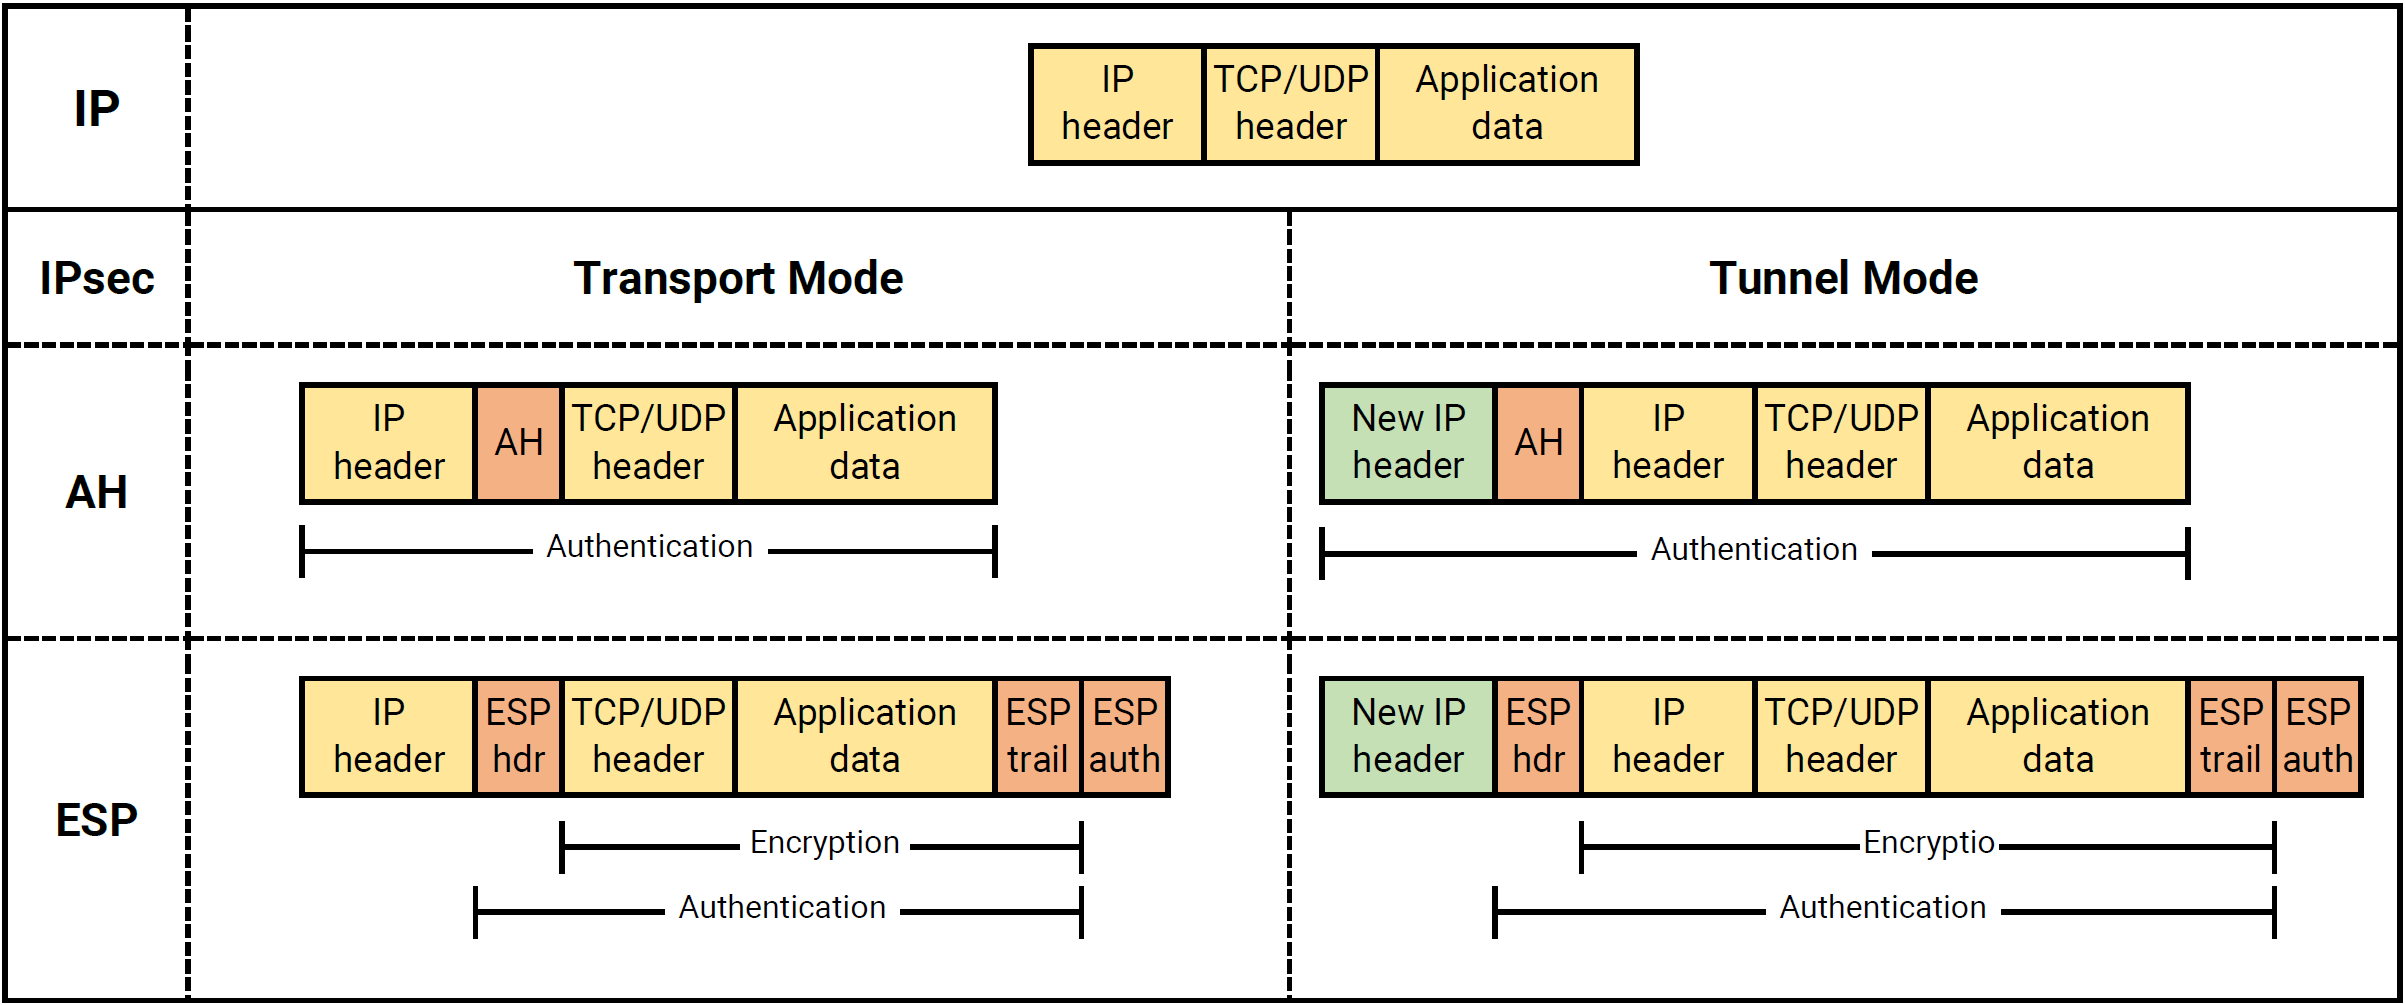
\includegraphics{image/ipsecmode.png}
    \caption{IPsec Mode of Operation}
    \label{fig:my_label}
\end{figure}

\begin{figure}[h]
\centering
\begin{subfigure}{.5\textwidth}
  \centering
  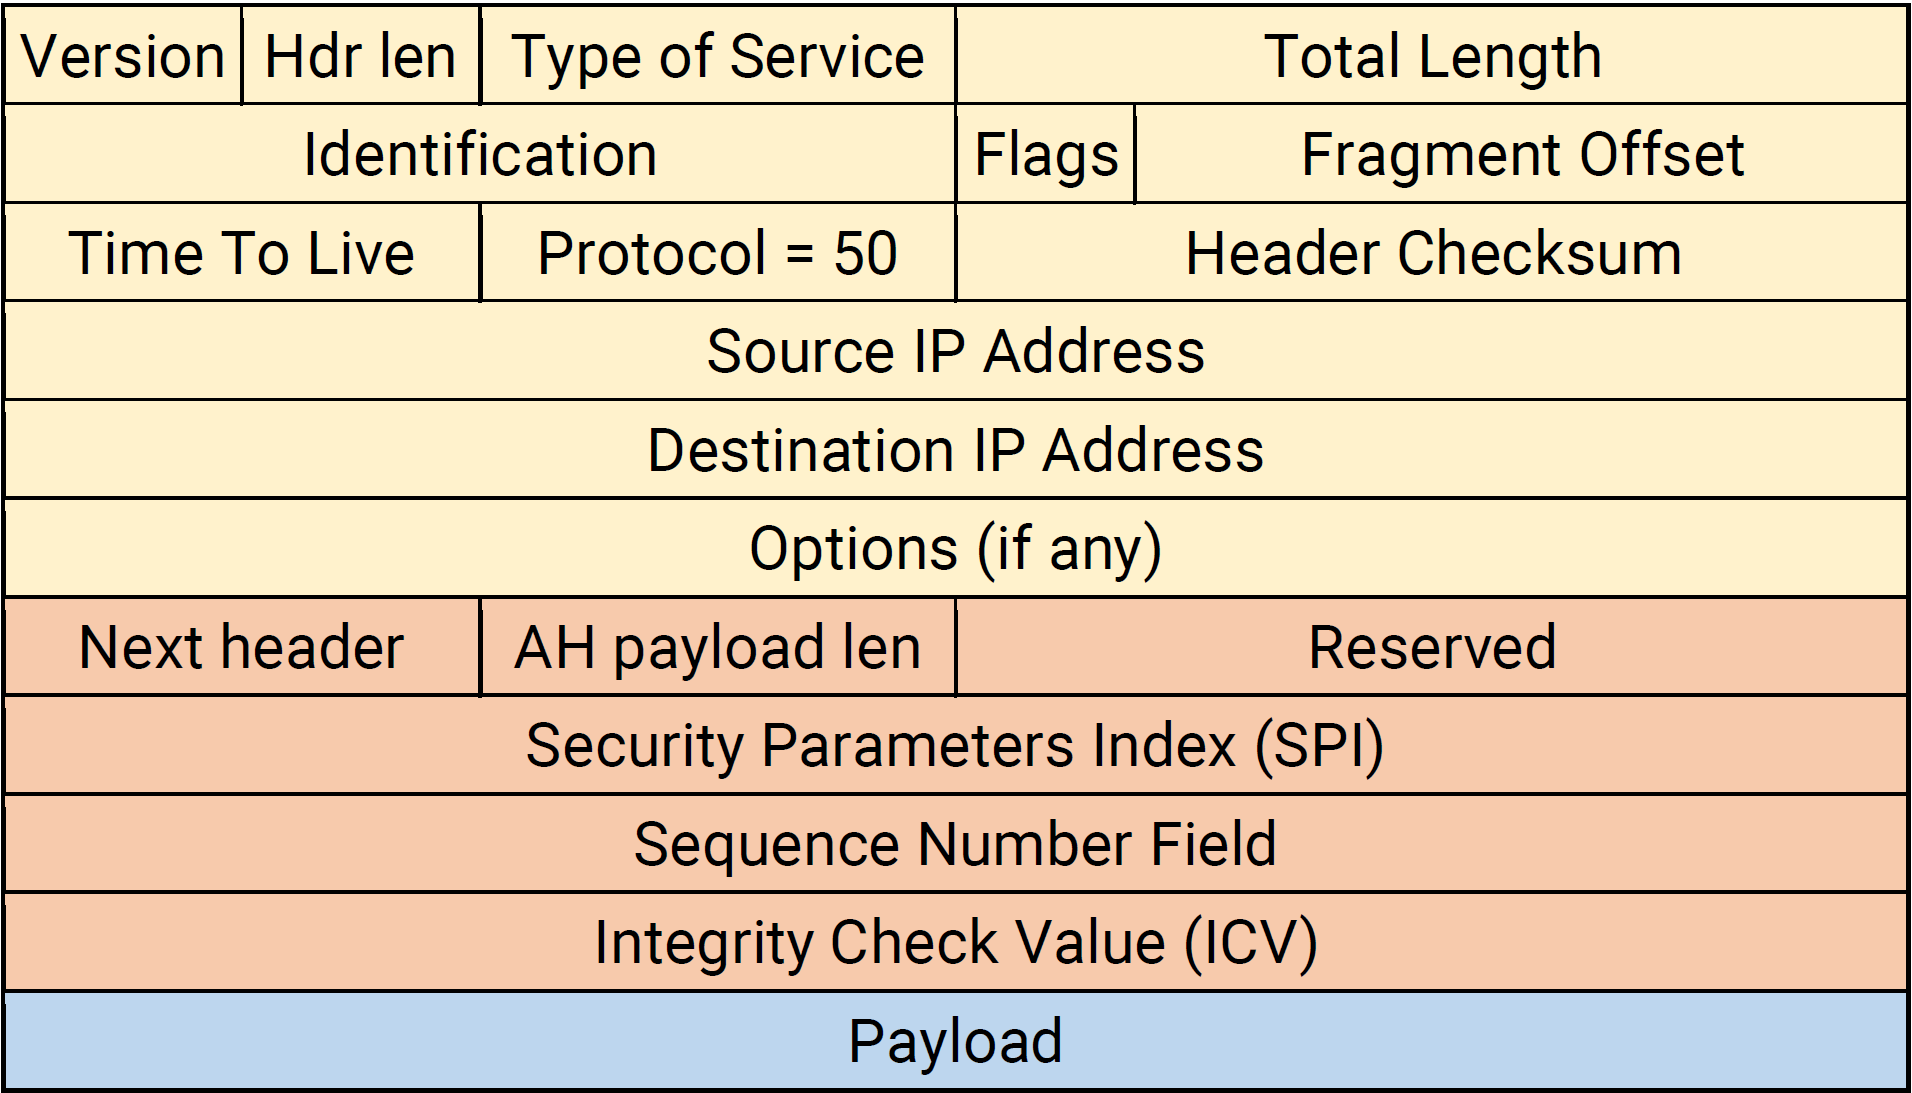
\includegraphics[width=0.99\textwidth]{image/ah.png}
  \caption{Authentication Header}
  \label{fig:ah}
\end{subfigure}%
\begin{subfigure}{.5\textwidth}
  \centering
  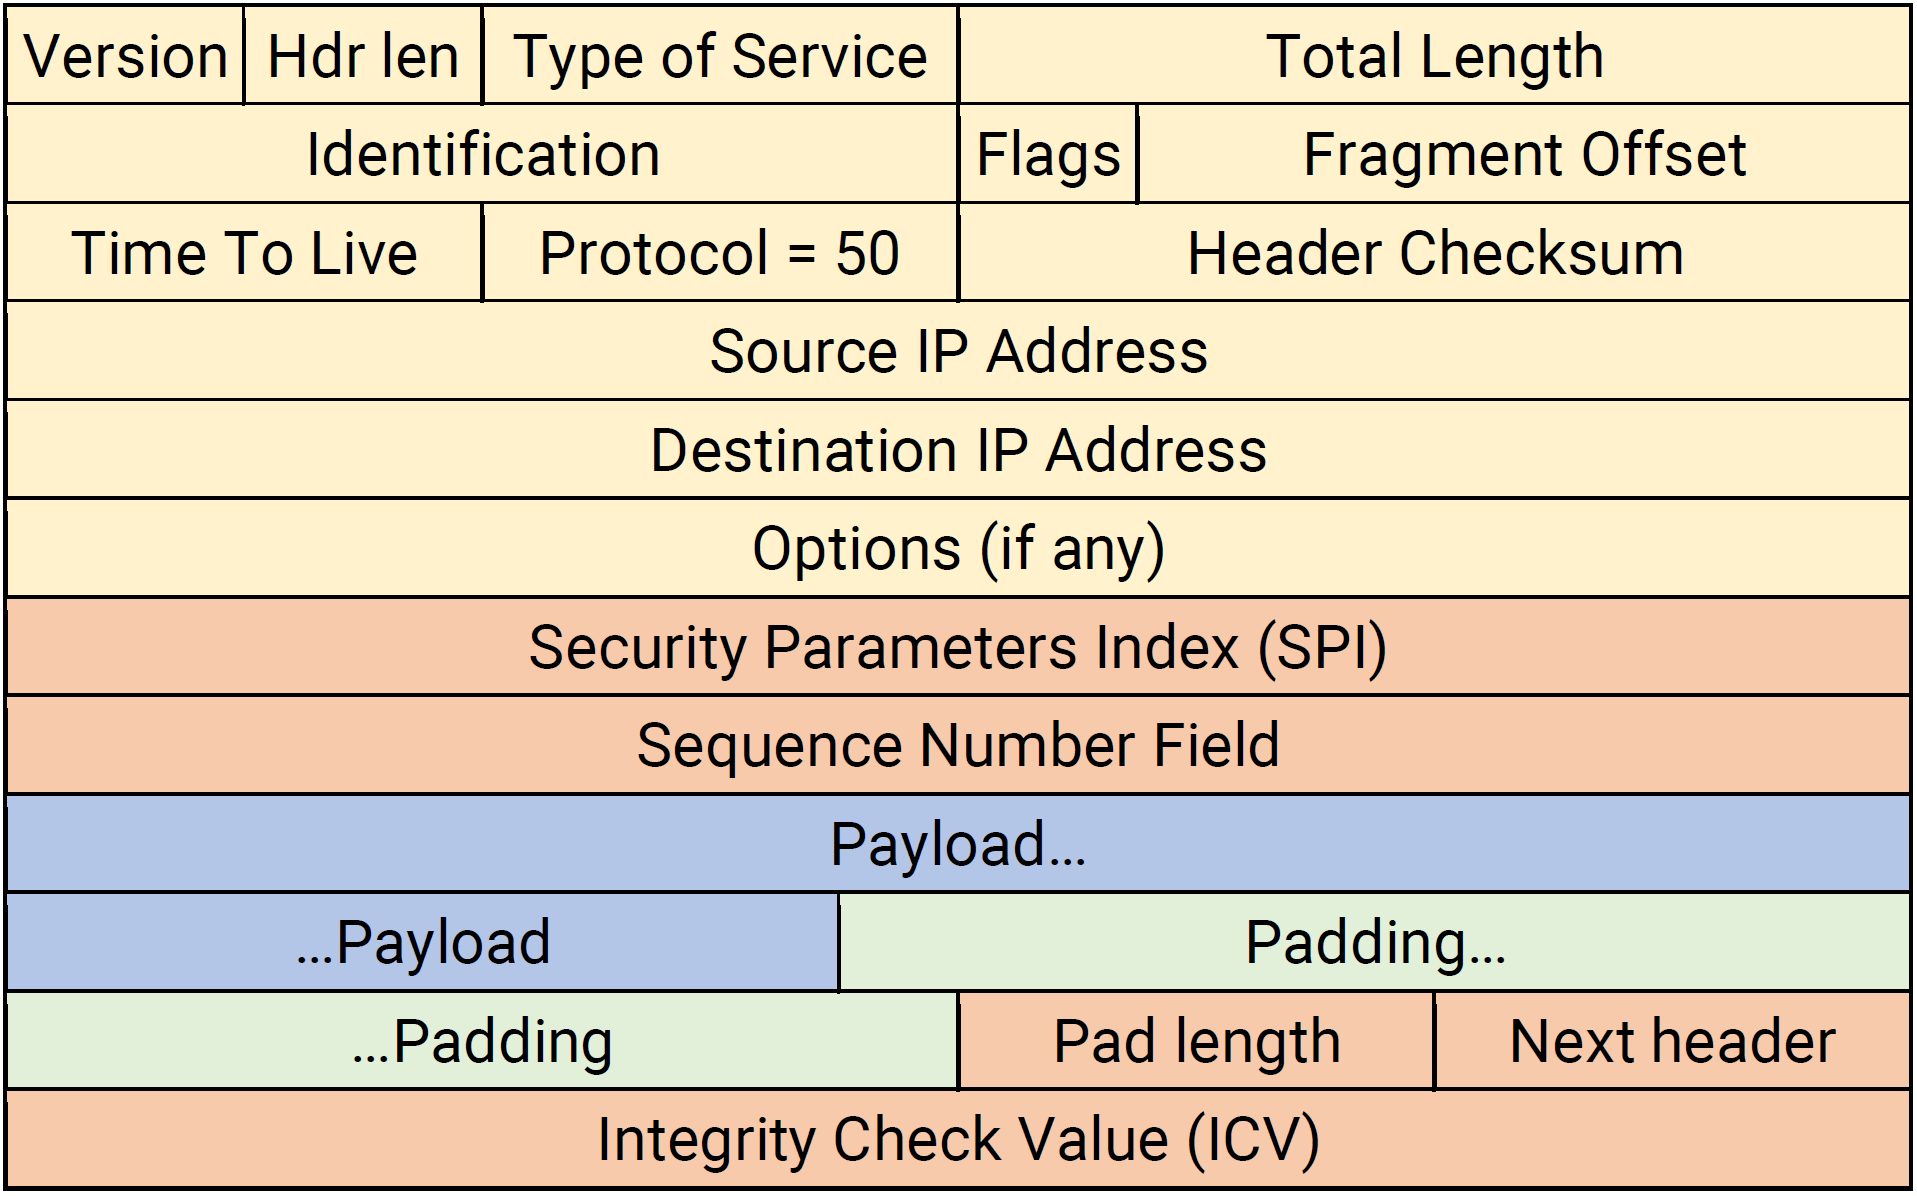
\includegraphics[width=0.99\textwidth]{image/esp.png}
  \caption{Encapsulated Security Payload}
  \label{fig:esp}
\end{subfigure}
\caption{IPsec Packet Format}
\label{fig:ipsecpktformat}
\end{figure}
L'integrità dei pacchetti viene controllata nel seguente modo:
\begin{theorem}[IPsec Integrity Check]\label{thm:ipsectag}
Viene generato un MAC contenuto nel campo \textbf{ICV (Integrity Check Value)}  nell'\textbf{header AH/trailer ESP} nel seguente modo:
\begin{itemize}
    \item Se viene usato AH, include tutti i \textbf{campi non mutabili/prevedibili} dell'header IP\footnotemark
    \footnotetext{\textsuperscript{\thefootnote}Ad esempio il Time-to-Live (TTL) e l'header checksum cambiano spesso. Per questi campi viene aggiunta una maschera di bit e poi calcolato il tag. Se viene usato AH, faccio MAC prima della frammentazione e ricontrollo al riassemblaggio.}
    \item Vengono inclusi per intero l'header \textbf{AH/ESP} ed il \textbf{payload IP}
\end{itemize}
\end{theorem}
\begin{note}
Al fine di proteggere IPsec da replay attacks sia AH che ESP usano un \textbf{extended sequence number (ESQN)} per numerare i pacchetti.
\end{note}
\begin{definition}[ESQN]\label{def:esqn}
Numero complessivamente di 64bit, di cui:
\begin{itemize}
    \item 32 bit \textbf{meno significativi} trasmessi con il \textbf{campo sequence number} nell'header AH/ESP.\footnotemark \footnotetext{\textsuperscript{\thefootnote}Il protocollo IP non prevede un campo apposito per tale funzione.}
    \item 32 bit \textbf{più significativi} mantenuti e aggiornati autonomamente dagli estremi.
    \item Viene sempre \textbf{inizializzato a 0} per una \textbf{nuova SA}
    \item Quando viene raggiunto il \textbf{massimo valore} esprimibile, la \textbf{SA viene terminata}.
\end{itemize}
\end{definition}
Viene poi introdotta una strategia anti-replay per determinare quali sequence number il destinatario reputa non validi.
\begin{theorem}[Anti-Replay Policy]\label{thm:antireplay}
Viene usata una \textbf{finestra scorrevole (sliding window)} così fatta:
\begin{itemize}
    \item La finestra (di ricezione) ha \textbf{dimensione W} definita dal ricevitore.
    \item Il \textbf{margine destro} è dato dal \textbf{numero di sequenza più alto ricevuto}. Poiché $W$ \textbf{fissato}, il margine sinistro è \textbf{univocamente determinato}.
    \item Alla \textbf{ricezione} di un \textbf{pacchetto} si applicano le seguenti regole:
    \begin{itemize}
        \item \textbf{Duplicato o a sinistra di W:} scarto il pacchetto.
        \item \textbf{All'interno di W e NON duplicato:} ricevo il pacchetto.
        \item \textbf{A destra di W} ed è contestualmente\footnotemark \textbf{possibile spostare in avanti W}: ricevo il pacchetto, altrimenti lo scarto.
        \footnotetext{\textsuperscript{\thefootnote}E' possibile \textbf{scorrere W in avanti di n posizioni} solamente se sono stati già ricevuti \textbf{tutti i pacchetti} nelle \textbf{prime n} posizioni di W.}
    \end{itemize}
\end{itemize}

\end{theorem}\pagebreak
\begin{note}
\textbf{E' stato osservato} che il \textbf{traffico prodotto durante la comunicazione} con un determinato server \textbf{possiede una firma statistica} che \textbf{permette di distinguerlo dagli altri} server. In particolare, esaminando le \textbf{proprietà dei pacchetti trasmessi} durante l’inizio di una nuova connessione con il server è possibile \textbf{tracciare} delle \textbf{caratteristiche} come:
\begin{itemize}
    \item \textbf{Dimensione dei pacchetti} scambiati.
    \item \textbf{Tempo} di  \textbf{inter-arrivo} tra i pacchetti.
    \item \textbf{Presenza} o \textbf{assenza} di determinati tipi di pacchetti.
\end{itemize}
\end{note}
Dalle firme statistiche del traffico, un attaccante può \textbf{determinare} con \textbf{quale server} il \textbf{client comunica}, solamente analizzando il traffico generato. \\
\begin{remark}
Sarebbe possibile generare dei collegamenti tra \textbf{client} e \textbf{server} che possono essere usati per strutturare attacchi più complessi.
\end{remark}
Introduciamo quindi un \textbf{nuovo} requisito di sicurezza.
\begin{definition}[Traffic Flow Confidentiality]\label{def:trafflow}
E' un servizio di sicurezza che ha come obiettivo l'\textbf{offuscamento} della \textbf{firma} del \textbf{traffico}
\end{definition} 
ESP ha due differenti meccanismi per contrastare l'analisi del traffico:
\begin{proposition}[ESP Traffic Flow Conf.]
\begin{itemize}
    \item E' possibile alterare la dimensione dei pacchetti aggiungendo del padding. 
    \begin{itemize}
        \item [\textcolor{green}{\checkmark}] facilmente gestibile utilizzando tunnel mode.
        \item [\textcolor{red}{\ding{55}}] Il padding TCF potrebbe indebolire gli algoritmi di criptazione.
    \end{itemize}
    \item E' possibile generare \textbf{pacchetti fantoccio} (dummy) da immettere 
\end{itemize}
\end{proposition}
\section{IKEv2 - Internet Key Exchange}
\begin{definition}[IKEv2]\label{def:ikev2}
Il \textbf{protocollo IKEv2 (Internet Key Exchange v2)} permette di creare \textbf{molteplici SA} in maniera \textbf{sicura} tra due peers/hosts. In particolare, si distinguono:
\begin{itemize}
    \item \textbf{Initiatior:} \textbf{host/peer} che \textbf{genera} ed \textbf{invia} una \textbf{richiesta}. In genere corrisponde con il client.
    \item \textbf{Responder:} \textbf{host/peer} che \textbf{riceve} una \textbf{richiesta IKE}. In genere corrisponde con il server.
    \item \textbf{IKE SA:} \textbf{Security Association} \textbf{creata ed utilizzata dal protocollo IKE} per messaggi di controllo. Ne viene \textbf{generata} solamente \textbf{una per istanza IKE}.
    \item \textbf{Child SA:} \textbf{Security Association creata} per \textbf{effettuare} lo \textbf{scambio dati tra i peers utilizzando il protocollo IPsec AH/ESP}. Da un’unica istanza del protocollo IKE possono essere create molteplici Child SA per servire scopi differenti.
\end{itemize}
\end{definition}\pagebreak
\subsection{Funzionamento}
Il protocollo IKE è strutturato in 2 fasi:
\begin{proposition}
\begin{enumerate}
    \item \textbf{Handshake 4-way:} viene create la \textbf{IKE SA} e vengono scambiati due tipi di messaggi:
\begin{itemize}
    \item \textbf{IKE SA Init:} messaggi in chiaro utilizzati per \textbf{negoziare} i \textbf{parametri IKE}\footnotemark
    \footnotetext{\textsuperscript{\thefootnote}Security Association Parameters: \textbf{SAP}} e \textbf{inviare} le \textbf{nonces} ed i \textbf{valori DH}\footnotemark
    \footnotetext{\textsuperscript{\thefootnote}Key Exchange Values \textbf{KE}}
    \item \textbf{IKE Auth:} \textbf{messaggi criptati simmetricamente} e \textbf{autenticati} per \textbf{confermare} l'avvenuta negoziazione. Permettono anche di \textbf{contrastare downgrade attacks}.
\end{itemize}
\item \textbf{Child SA:} (opzionale) vengono create delle SA child e vengono inviati messaggi IKE di \textbf{controllo}.
\end{enumerate}
\end{proposition}
\begin{figure}[h]
    \centering
    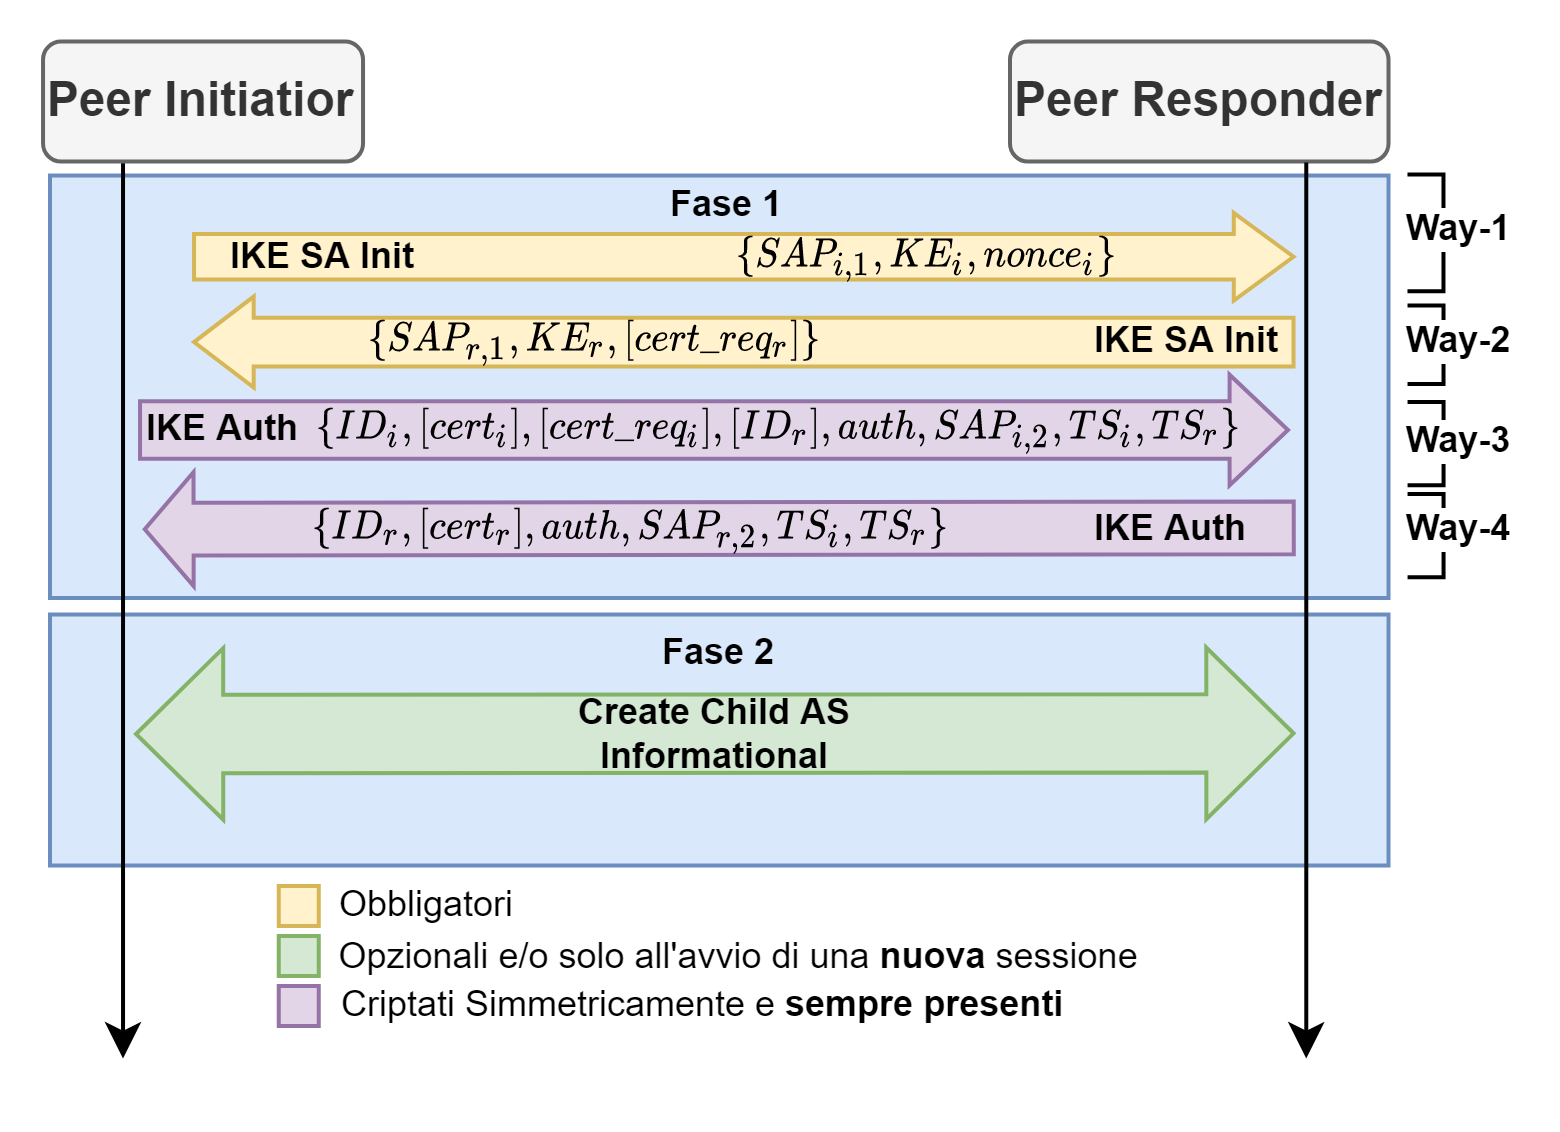
\includegraphics[width=0.9\textwidth]{image/ikev2.png}
    \caption{IKE 4-way Handshake}
    \label{fig:ikev2}
\end{figure}
\pagebreak
I messaggi hanno il seguente formato:
\begin{definition}[IKE Msg Format]\label{def:ikemsg}
\begin{itemize}
    \item \textbf{IKE Header:} indica il tipo di messaggio IKE.
    \item \textbf{IKE Payloads:} lista collegata di payload differenti. Ogni singolo payload possiede un proprio formto ed una propria funzione. Tale \textbf{struttura flessibile} permette di \textbf{estendere} rapidamente un \textbf{messaggio} IKE e, di fatto, le \textbf{funzionalità} del \textbf{protocollo IKE} stesso.
\end{itemize}
\begin{remark}
Questi messaggi sono trasportati tramite \textbf{UDP}, \textbf{reso affidabile} dal protocollo IKE stesso, ed \textbf{inviati} tramite protocollo IP.
\end{remark}
\end{definition}
\subsection{Key Computation}
\begin{note}
Nelle versioni più recenti vengono usate \textbf{solo HKDF} in quanto più sicure. Vediamo però come venivano costruite:
\end{note}
Le chiavi della \textbf{sessione IKE} vengono generate anche queste con approccio \textit{\textbf{Extract-than-Expand}} \cref{def:ete} tramite delle \textbf{PRF Negoziate} nella fase 1, utilizzando le \textbf{nonces} e i \textbf{dh coefficient} scambiati con i \textbf{messaggi di IKE SA Init}. 
\begin{definition}[IKE Key Computation]
\begin{itemize}
    \item \textbf{Extract:}$SK_{seed}=PRF(nonce_i,nonce_r,g^{ir})$\footnotemark
    \footnotetext{\textsuperscript{\thefootnote}$g^{ir}$ è il DH shared key.}
    \item \textbf{Expand:}$\text{Keys}=PRF^+(SK_{seed},nonce_i,nonce_r,SPI_i,SPI_r)$
\end{itemize}
E vengono generate 7 chiavi di sessione:
\begin{itemize}
    \item $SK_{ai},SK_{ar}$ per il controllo di integrità.
    \item $SK_{ei},SK_{er}$ per encryption e decryption.
    \item $SK_{pi},SK_{pr}$ per la \textbf{generazione} di un \textbf{AUTH payload} nella fase SA\_AUTH.
    \item $SK_{d}$ per la derivazione di ulteriori chiavi per le \textbf{Child\_SA}.
\end{itemize}
\end{definition}
\section{Vulnerabilità}
IPsec non è immune ad attacchi e qui ne consideriamo due tipi:
\begin{itemize}
    \item Downgrade Attacks
    \item DoS Attacks
\end{itemize}
Vediamo come IPsec si è protetto da questi attacchi.
\subsection{Against Downgrade Attack}
Viene \textbf{introdotto} un \textbf{version flag $V$} in \textbf{tutti} i messaggi scambiati. Tale flag indica se la \textbf{versione del protocollo negoziata} non è quella \textbf{massima disponibile.}
\begin{definition}[IPsec Version Flag]\label{def:versionflag}
\begin{itemize}
    \item \textbf{$V=0$} se il \textbf{mittente} del messaggio sta \textbf{negoziando} la propria \textbf{versione massima}.
    \item \textbf{$V=1$} altriment, ovvero se il \textbf{mittente} del messaggio sta \textbf{negoziando} una \textbf{versione inferiore alla propria versione massima disponibile.}
\end{itemize}
\end{definition}
Un attaccante MITM può modificare sia la versione che il version flag all'interno dei messaggi di IKE SA Init per effettuare un downgrade. Tuttavia, l'attaccante non potrà alterare i messaggi di IKE SA Auth nel quale è contenuto il version flag realmente dichiarato, poiché protetti tramite criptazione e autenticazione.\\
\begin{remark}
SIa l'initiator che il responder possono \textbf{rilevare l'attacco} semplicemente \textbf{verificando} che i \textbf{version flag} sono per \textbf{entrambi} pari a $1$, ovvero, \textbf{nessuno dei due sta utilizzando la propria versione massima}. La versione ottima per la sicurezza è infatti data dalla minima tra le due versioni massime disponibili.
\end{remark}
\begin{figure}[h]
    \centering
    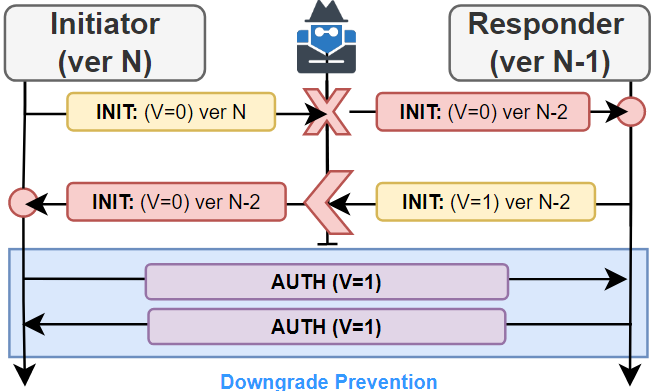
\includegraphics[width=0.8\textwidth]{image/ikedown.png}
    \caption{Downgrade Attack and Prevention in IKEv2}
    \label{fig:ikedown}
\end{figure}\pagebreak
\subsection{Against DoS Attacks}
Il \textbf{DoS (Denial of Service)} \textbf{attack} utilizza delle \textbf{spoofed IKE SA Init} per \textbf{saturare} le \textbf{capacità computazionali} del \textbf{server} e renderlo \textbf{inaccessibile} agli utenti legittimi. Nel caso del protocollo IKE viene sfruttata l’\textbf{onerosità delle computazioni DH} svolte \textbf{dopo} i primi due \textbf{messaggi} di \textbf{IKE SA Init}.\\
Il protocollo IKE viene protetto da DoS attack utilizzando un \textbf{Init handshake 4-way} basato sull’uso di \textbf{cookie}. In particolare, vengono inviati i seguenti messaggi
\begin{definition}[IKE DoS Prevention]
\textbf{Prima dell'init} vengono \textbf{aggiunti} due messaggi:
\begin{enumerate}
    \item \textbf{Request:} il client invia la \textbf{richiesta} di connessione al server.
    \item \textbf{Response:} il server risponde al client \textbf{ripetendo} a richiesta ed inviando un \textbf{cookie}.
    \item \textbf{IKE SA Init (Initiator)}: il client deve rispondere con un messaggio IKE SA Init in cui ripete la richiesta ed il cookie appena ricevuto dal server.
    \item \textbf{IKE SA Init (Responder)}: se la richiesta ed il cookie all’interno del messaggio IKE SA Init ricevuto corrispondono con quelli dei messaggi precedenti, il server continua con il protocollo IKE.
\end{enumerate}
Il server inizia le elaborazioni solamente al termine dell’Init handshake. 
\end{definition}
\begin{note}
Tale schema permette di \textbf{contrastare attacchi DoS basati su IP spoofing} in quanto l’\textbf{attaccante non riceve} il messaggio di \textbf{Response}, indirizzato verso l’indirizzo IP spoofed diverso dal suo, e non quindi può continuare l’handshake.
\end{note}
\begin{corollary}[Cookie for Handshake 4-way]
I \textbf{cookie} devono essere stateless: \textbf{casuali, non ripetuti e non predicibili}. Sono possibili due approcci:
\begin{itemize}
    \item \textbf{Generazione Diretta:} i cookie vengono generati come stringe casuali.
    \begin{itemize}
        \item \textbf{Poco Scalabile} in termini di \textbf{memoria}, in quanto occorre memorizzare tutti i cookie generati in precedenza per evitare di effettuare ripetizioni.
        \item \textbf{E' prono ad errori implementativi} per i quali i cookie vengono ripetuti o sono predicibili.
    \end{itemize}
    \item \textbf{Generazione} tramite \textbf{funzione hash:} $\text{cookie}=H_k(request)$
    \begin{itemize}
        \item I cookie vengono generati usando una funzione hash crittografica $H$, una chiave segreta $K$, nota solamente al server e l'intero messaggio di richiesta per i quali vengono generati.\\
        Corrispondono al MAC per la message authentication dei messaggi.
        \item La \textbf{chiave segreta K} può essere \textbf{cambiata periodicamente} per fornire \textbf{maggiore robustezza}.
    \end{itemize}
\end{itemize}
\end{corollary} 
\begin{figure}[H]
\centering
\begin{subfigure}{\textwidth}
  \centering
  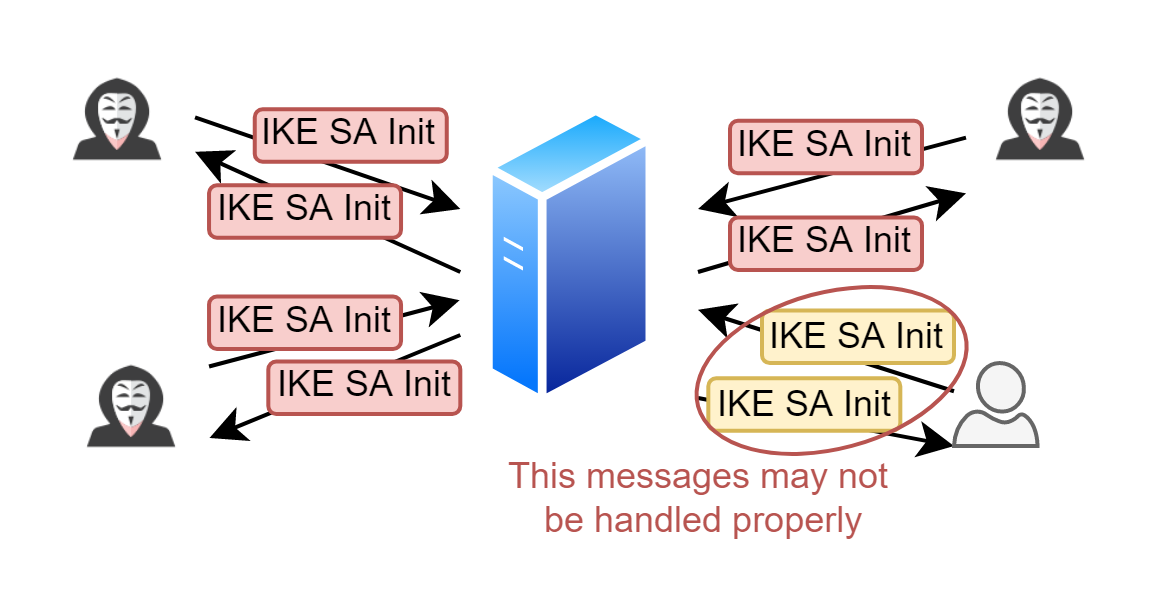
\includegraphics[width=0.99\textwidth]{image/ikedos.png}
  \caption{(D)DoS Attack}
  \label{fig:ikedos}
\end{subfigure}\\
\begin{subfigure}{\textwidth}
  \centering
  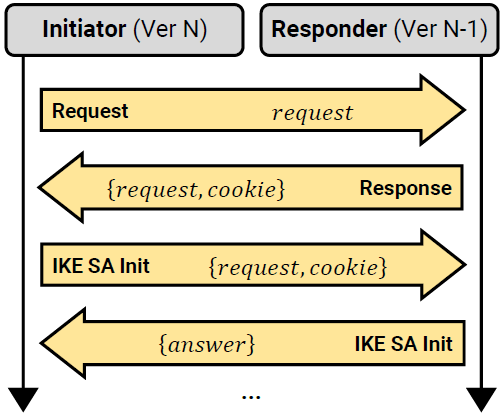
\includegraphics[width=0.7\textwidth]{image/ikedosprevent.png}
  \caption{4-way Handshake with Request and Response}
  \label{fig:ikedosprev}
\end{subfigure}
\end{figure}
\pagebreak
\section{VPN}
Una \textbf{Virtual Private Network} è una \textbf{rete virtuale privata} all'interno della rete pubblica che permette di 
\begin{itemize}
    \item \textbf{Proteggere} i \textbf{dati} \textbf{in transito nella VPN} dal resto della rete.
    \item \textbf{Connettere} in \textbf{maniera sicura} delle \textbf{sottoreti} geograficamente \textbf{distanti} tra loro.
\end{itemize}
Una VPN funziona con due meccanismi fondamentali:
\begin{itemize}
    \item \textbf{Tunneling:} \textbf{incapsulare/trasportare pacchetti IP}, relativi alla \textbf{LAN}, all'interno di altri pacchetti IP, relativi alla WAN.
    \item \textbf{Encryption:} \textbf{criptare} il \textbf{payload} di pacchetti IP e quindi, \textbf{nel caso venga usato il tunneling}, criptare per \textbf{intero un pacchetto IP.}
\end{itemize}
Una VPN può chiaramente essere realizzata usando IPsec in modalità Tunnel (\cref{def:tunnel}).
\begin{figure}[h]
    \centering
    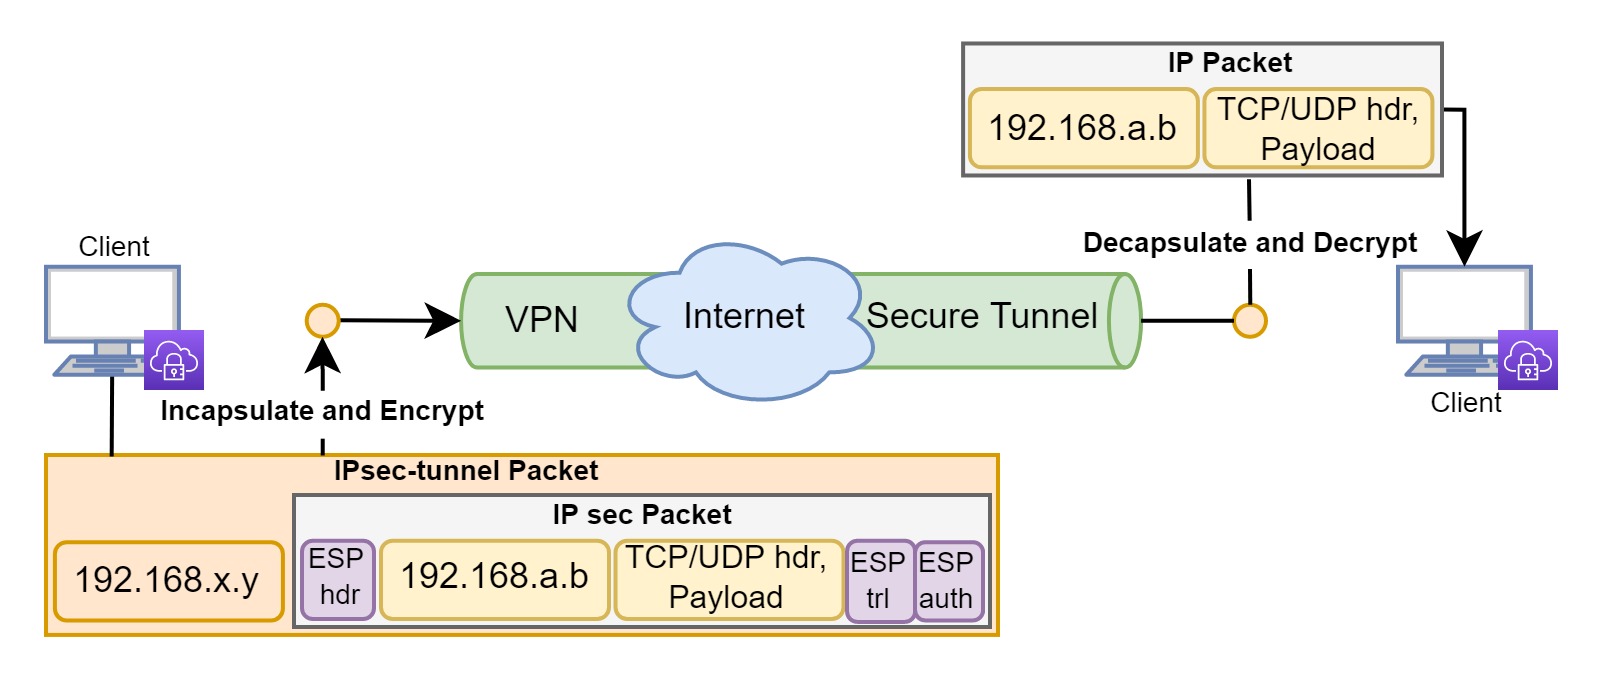
\includegraphics{image/vpn.png}
    \caption{VPN Scheme}
    \label{fig:vpn}
\end{figure}